%!TEX root = ../../ClassicThesis.tex
% =============================================================================
\section{Introduction}
% =============================================================================

In \autoref{ch:lam}, we considered the information in the power of the \ac{CSD} within different frequency ranges.
In this chapter, we will investigate the information encoded in the phase of the \ac{CSD}, and its relationship with the power.


% =============================================================================
\section{Methods}
% =============================================================================


\subsection{Phase across depth and frequencies}
\label{sec:lam_phase_method}

The phase was computed in a similar manner to the power in \autoref{sec:lam_power_method}.
We filtered both the \ac{LFP} and \ac{CSD} using a series of bands each with a fractional bandwidth of \SI{50}{\percent}, spaced logarithmically at multiples \num{1.291}.
This spacing ensures each band has \SI{0}{\percent} overlap with bands further away than its immediate neighbours and a \SI{44}{\percent} and \SI{56}{\percent} overlap with its preceding and succeeding bands respectively.
The filter chosen was a zero-phase sixth-order Butterworth filter, after which the instantaneous phase was estimated by taking the angle of the Hilbert transform.
The phase the \SIrange{4}{16}{Hz} and \SIrange{60}{170}{Hz} bands was extracted in the same manner.


\subsection{Information contained in cortical oscillation phase}
\label{sec:lam_phase_method}

Similar to \autoref{sec:lam_info_method}


\subsection{Phase-phase correlation}

We used directional (or circular) statistics
Circular statistics were computed using the CircStat toolbox \citep{Berens2009}.


\subsection{Phase-power correlation}

Circular statistics were computed using the CircStat toolbox \citep{Berens2009}.


\subsection{Cross-frequency phase-amplitude coupling}

Strength of cross-frequency coupling was measured using the Modulation Index \citep{Tort2010}.
\ac{CSD} data was filtered for two bands, \SIrange{4}{16}{Hz} and \SIrange{60}{170}{Hz}, using a zero-phase sixth-order Butterworth filter, and the instantaneous phase of \SIrange{4}{16}{Hz} and envelope amplitude of \SIrange{60}{170}{Hz} were each estimated using a Hilbert transform.
We took a histogram of the \SIrange{4}{16}{Hz} phase datapoints with \num{16} bins each of width $\nicefrac{\pi}{8}$ radians, and took the average of the \SIrange{60}{170}{Hz} amplitudes simultaneous with the phase datapoints in each bin.
This provides a distribution of amplitude at one depth as a function of phase at another.
The Modulation Index is then the normalised Kullback-Leibler divergence of this distribution from a uniform distribution.


% =============================================================================
\section{Results}
% =============================================================================


%-------------------------------------------------------------------------------
\FloatBarrier
\subsection{Information contained in phase of cortical oscillations}

Again, although it contains less information than the \ac{LFP}, the \ac{CSD} gives better spatial localisation.

\begin{figure}[htbp]
    \centering
    \hspace*{\fill}
    \subfloat[\ac{LFP} phase information.\label{fig:lam_phase_info_lfp}]{
        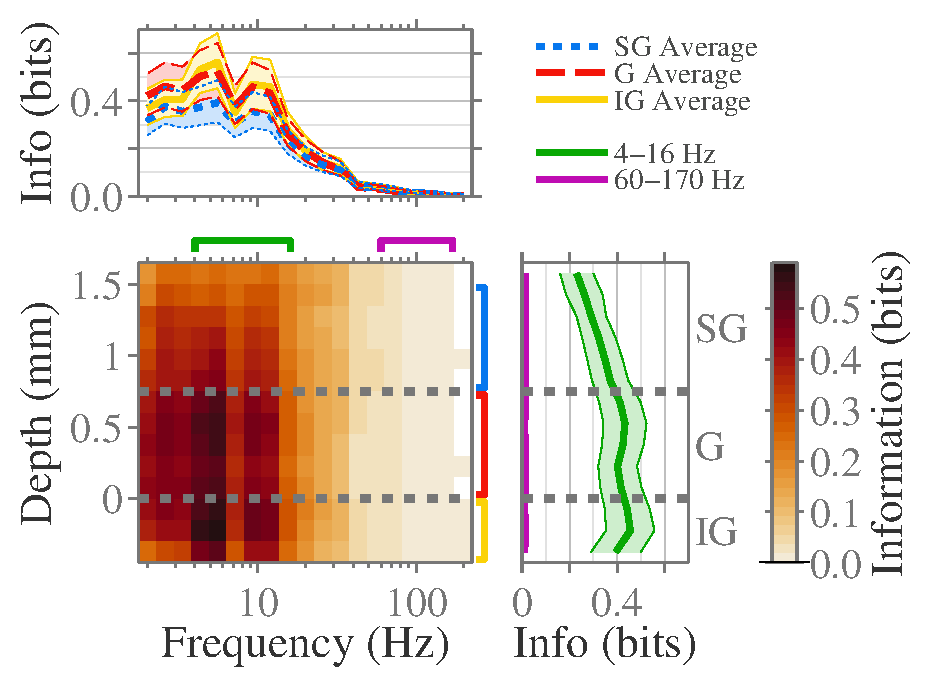
\includegraphics[scale=.45]{phaseinfo/fig3set-info-Cln-phase-straightnanmean-compzonescb-legend.eps}}
    \hspace*{\fill}\hspace{.2cm}\hspace*{\fill}
    \subfloat[\ac{CSD} phase information.\label{fig:lam_phase_info_csd}]{
        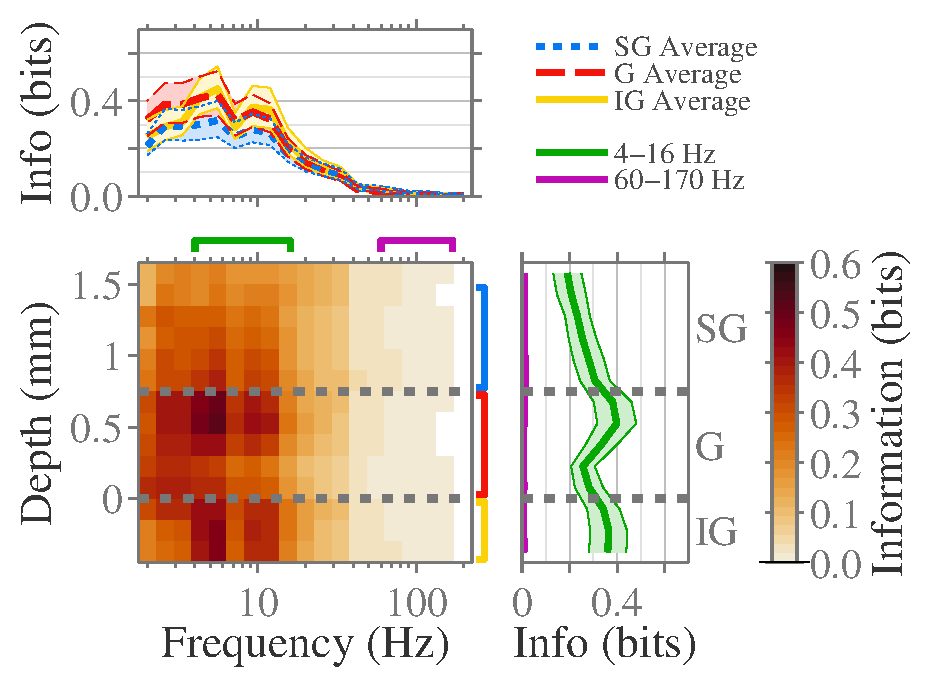
\includegraphics[scale=.45]{phaseinfo/fig3set-info-Csd-phase-straightnanmean-compzonescb-legend.eps}}
    \hspace*{\fill}
    \caption{
Information about the stimulus contained in the phase of the extracellular neural signal, as a function of frequency. Mean of 6 sessions.
\protect\subref{fig:lam_phase_info_lfp}:~\ac{LFP}.
\protect\subref{fig:lam_phase_info_csd}:~\ac{CSD}.
}
\label{fig:lam_phase_info}
\end{figure}


% \begin{figure}[htbp]
%     \centering
%     \hspace*{\fill}
%     \subfloat[\sesname{H05391}\label{fig:lam_phase_info_lfp_H05391}]{
%         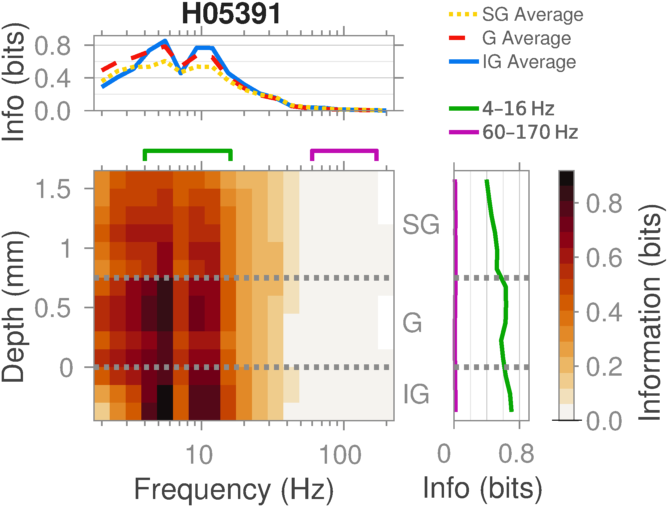
\includegraphics[scale=.4]{phaseinfo/fig3set-info-Cln-phase-H05391-compzonescb-legend.png}
% }
%     \hspace*{\fill}\hspace{.2cm}\hspace*{\fill}
%     \subfloat[\sesname{H05nm9}\label{fig:lam_phase_info_lfp_H05nm9}]{
%         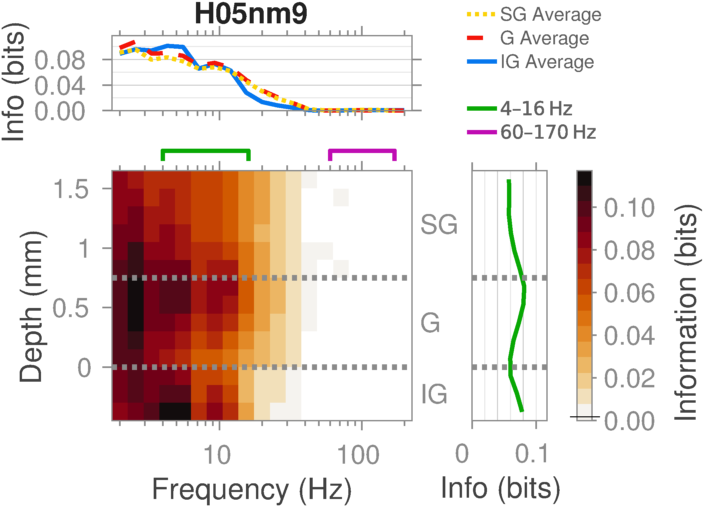
\includegraphics[scale=.4]{phaseinfo/fig3set-info-Cln-phase-H05nm9-compzonescb-legend.png}
% }
%     \hspace*{\fill}
%     \\
%     \hspace*{\fill}
%     \subfloat[\sesname{H05nm7}\label{fig:lam_phase_info_lfp_H05nm7}]{
%         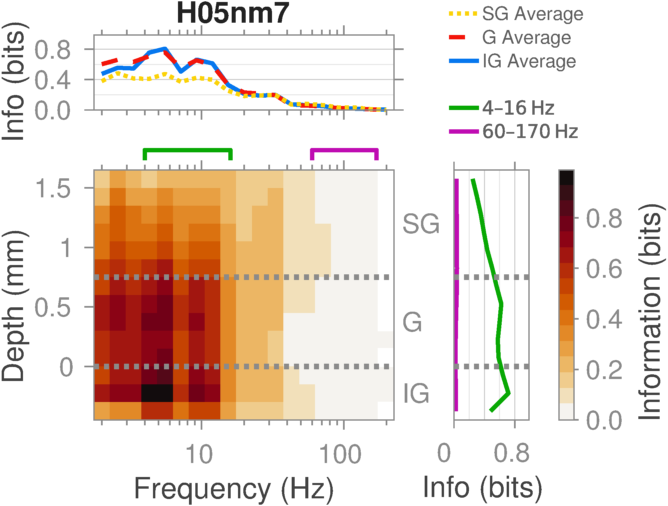
\includegraphics[scale=.4]{phaseinfo/fig3set-info-Cln-phase-H05nm7-compzonescb-legend.png}
% }
%     \hspace*{\fill}\hspace{.2cm}\hspace*{\fill}
%     \subfloat[\sesname{E07nm1}\label{fig:lam_phase_info_lfp_E07nm1}]{
%         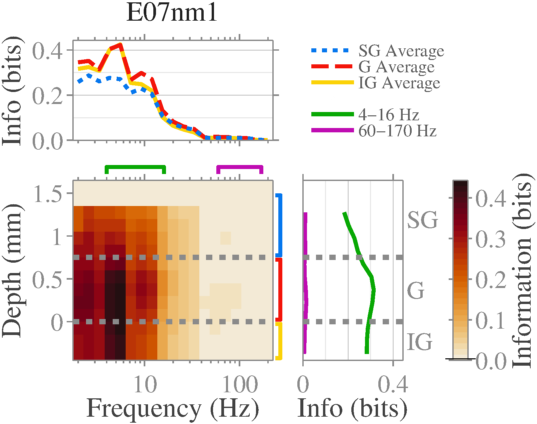
\includegraphics[scale=.4]{phaseinfo/fig3set-info-Cln-phase-E07nm1-compzonescb-legend.png}
% }
%     \hspace*{\fill}
%     \\
%     \hspace*{\fill}
%     \subfloat[\sesname{F10nm1}\label{fig:lam_phase_info_lfp_F10nm1}]{
%         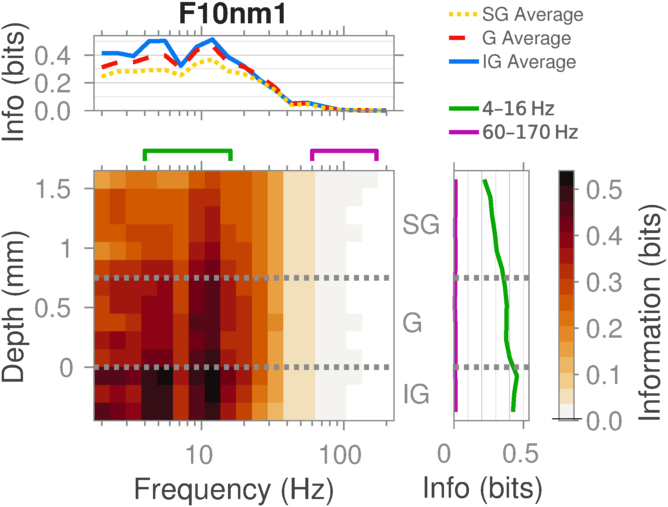
\includegraphics[scale=.4]{phaseinfo/fig3set-info-Cln-phase-F10nm1-compzonescb-legend.png}
% }
%     \hspace*{\fill}\hspace{.2cm}\hspace*{\fill}
%     \subfloat[\sesname{J10nm1}\label{fig:lam_phase_info_lfp_J10nm1}]{
%         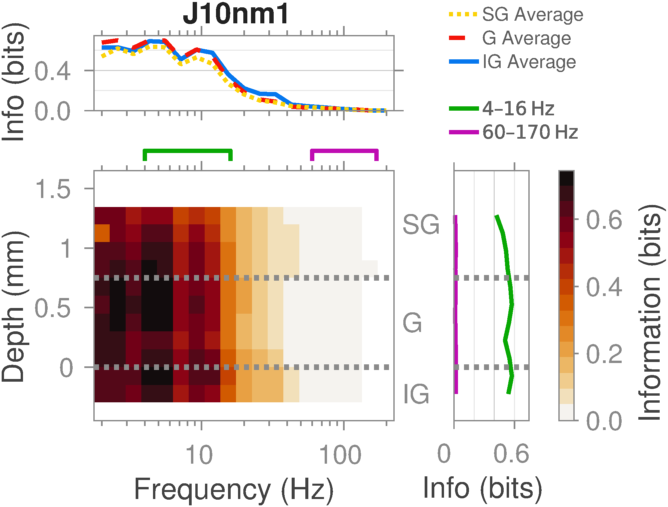
\includegraphics[scale=.4]{phaseinfo/fig3set-info-Cln-phase-J10nm1-compzonescb-legend.png}
% }
%     \hspace*{\fill}
%     \caption{
% Information about the stimulus contained in the phase of the \ac{LFP}, as a function of frequency, by session.
% }
% \label{fig:lam_phase_info_lfp_sessions}
% \end{figure}


% \begin{figure}[htbp]
%     \centering
%     \hspace*{\fill}
%     \subfloat[\sesname{H05391}\label{fig:lam_phase_info_csd_H05391}]{
%         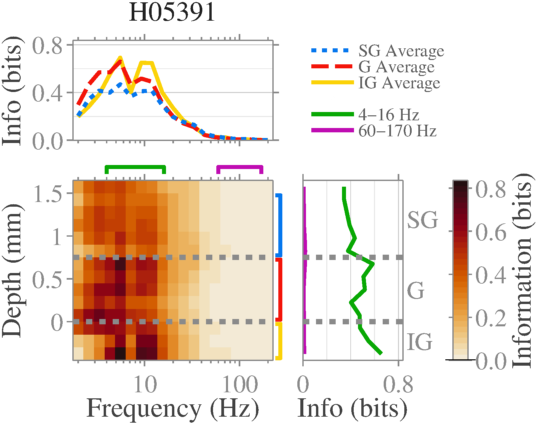
\includegraphics[scale=.4]{phaseinfo/fig3set-info-Csd-phase-H05391-compzonescb-legend.png}
% }
%     \hspace*{\fill}\hspace{.2cm}\hspace*{\fill}
%     \subfloat[\sesname{H05nm9}\label{fig:lam_phase_info_csd_H05nm9}]{
%         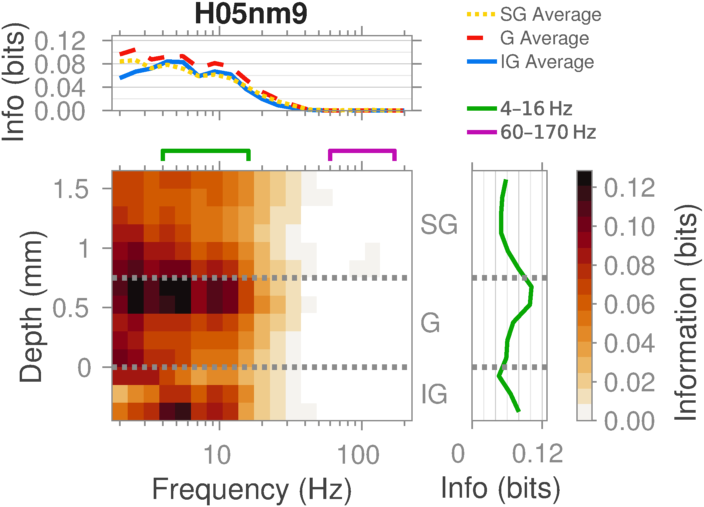
\includegraphics[scale=.4]{phaseinfo/fig3set-info-Csd-phase-H05nm9-compzonescb-legend.png}
% }
%     \hspace*{\fill}
%     \\
%     \hspace*{\fill}
%     \subfloat[\sesname{H05nm7}\label{fig:lam_phase_info_csd_H05nm7}]{
%         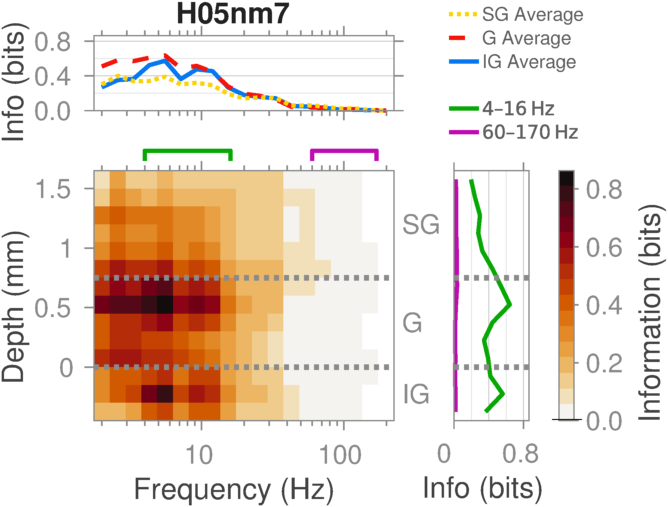
\includegraphics[scale=.4]{phaseinfo/fig3set-info-Csd-phase-H05nm7-compzonescb-legend.png}
% }
%     \hspace*{\fill}\hspace{.2cm}\hspace*{\fill}
%     \subfloat[\sesname{E07nm1}\label{fig:lam_phase_info_csd_E07nm1}]{
%         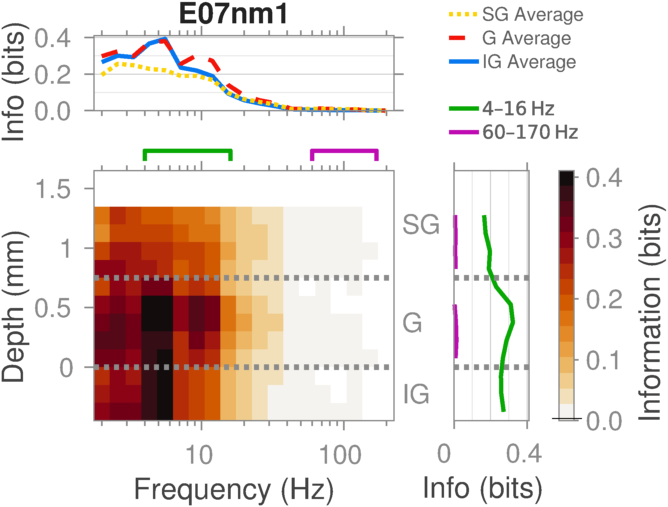
\includegraphics[scale=.4]{phaseinfo/fig3set-info-Csd-phase-E07nm1-compzonescb-legend.png}
% }
%     \hspace*{\fill}
%     \\
%     \hspace*{\fill}
%     \subfloat[\sesname{F10nm1}\label{fig:lam_phase_info_csd_F10nm1}]{
%         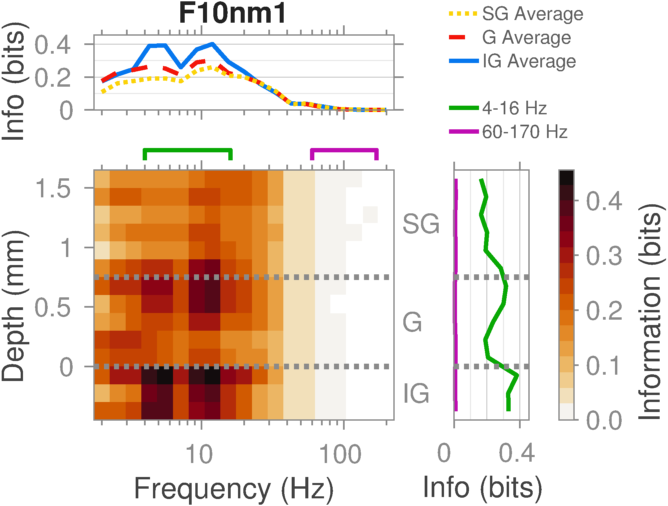
\includegraphics[scale=.4]{phaseinfo/fig3set-info-Csd-phase-F10nm1-compzonescb-legend.png}
% }
%     \hspace*{\fill}\hspace{.2cm}\hspace*{\fill}
%     \subfloat[\sesname{J10nm1}\label{fig:lam_phase_info_csd_J10nm1}]{
%         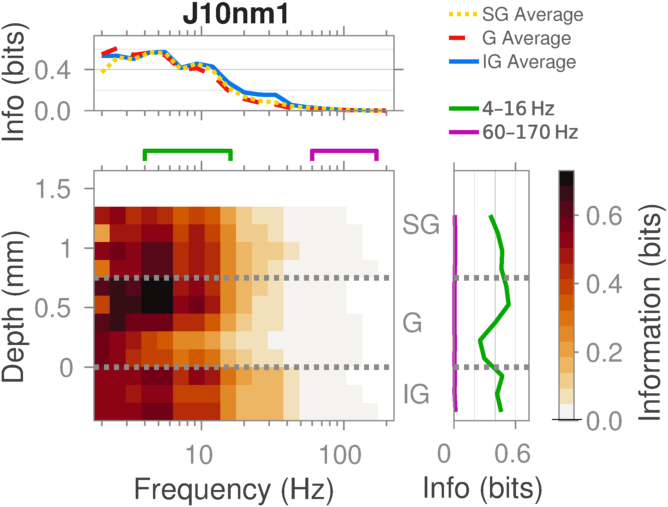
\includegraphics[scale=.4]{phaseinfo/fig3set-info-Csd-phase-J10nm1-compzonescb-legend.png}
% }
%     \hspace*{\fill}
%     \caption{
% Information about the stimulus contained in the phase of the \ac{CSD}, as a function of frequency, by session.
% }
% \label{fig:lam_phase_info_csd_sessions}
% \end{figure}


%-------------------------------------------------------------------------------
\subsection{Phase-phase redundancy}
%-------------------------------------------------------------------------------

We find that different frequency bands contain independent, or even synergistic, information about the stimulus.

\begin{figure}[htbp]
\centering
\hspace*{\fill}
\subfloat[Redundancy.\label{fig:lam_phase_cxfrq_info_red}]{
    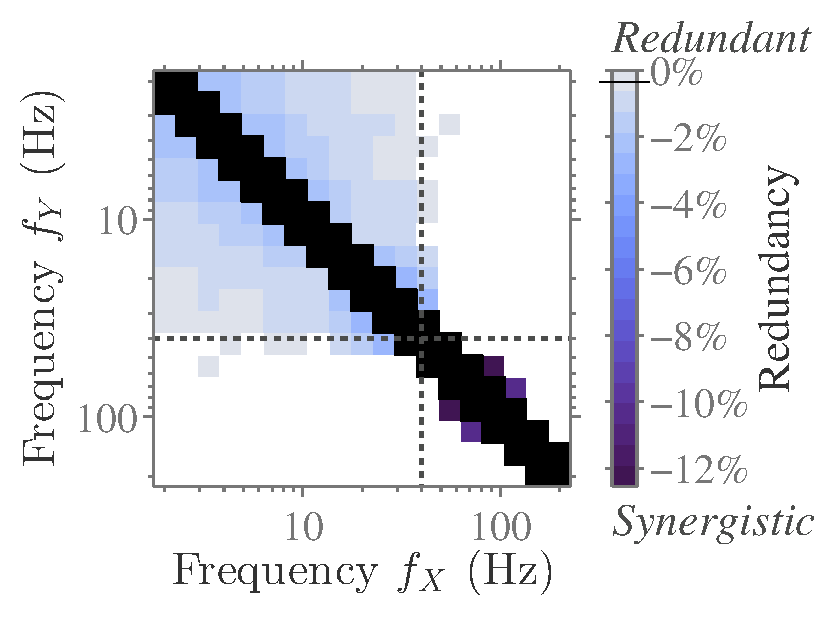
\includegraphics[scale=.5]{%
redundancy-cxsfrq/cxsfrq-pcred_phase-phase_avg-log_nodiag.eps}}
\hspace*{\fill}\hspace{.2cm}\hspace*{\fill}
\subfloat[Info gain.\label{fig:lam_phase_cxfrq_info_gain}]{
    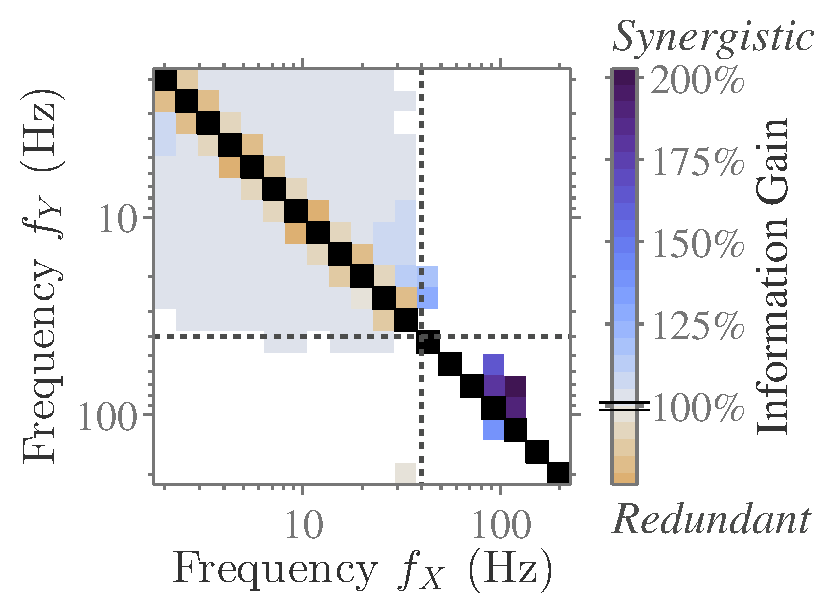
\includegraphics[scale=.5]{%
redundancy-cxsfrq/cxsfrq-pcgain-i2d2_phase-phase_avg-log_nodiag.eps}}
\hspace*{\fill}
    \caption{
Redundancy between frequencies.
}
\label{fig:lam_phase_cxfrq_info}
\end{figure}

\begin{figure}[htbp]
    \centering
    \hspace*{\fill}
    \subfloat[Signal correlation\label{fig:lam_signal_corr_phase}]{
        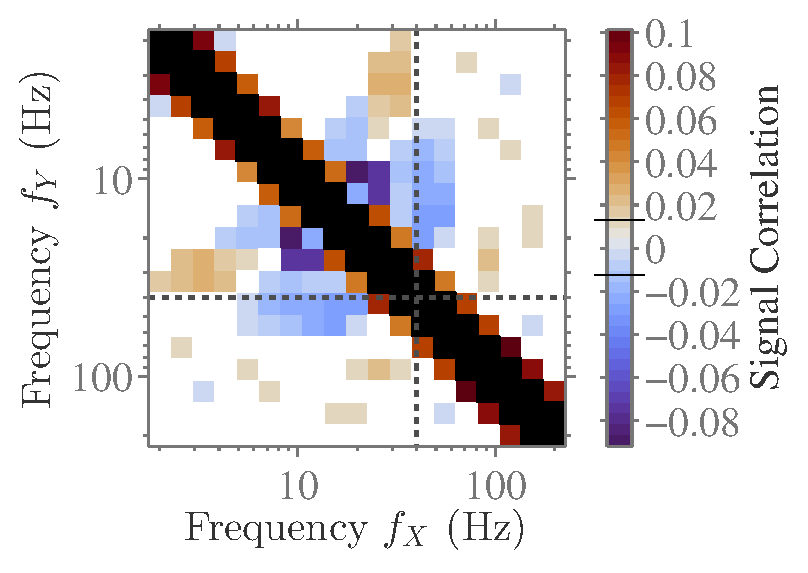
\includegraphics[scale=.5]{noisesigcorr/cxsfrq-signal-phase-phase-avg-log_nodiag.eps}
}
    \hspace*{\fill}\hspace{.2cm}\hspace*{\fill}
    \subfloat[Noise correlation\label{fig:lam_noise_corr_phase}]{
        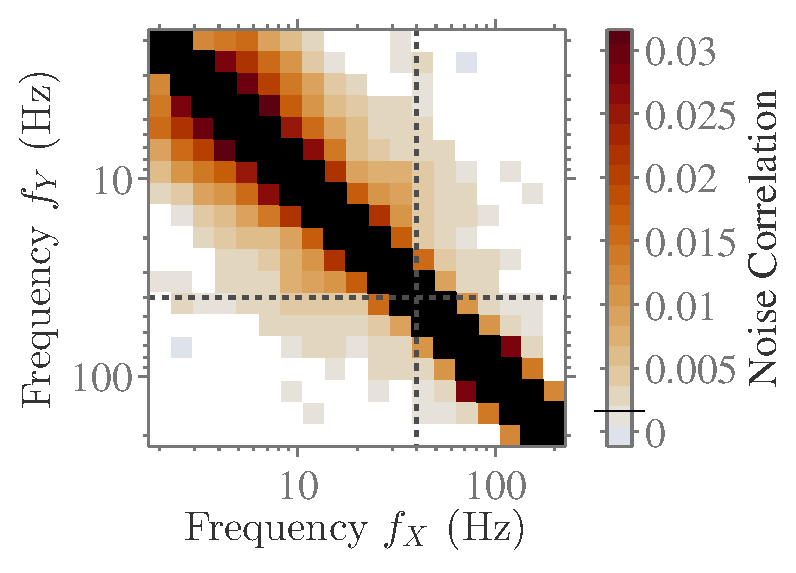
\includegraphics[scale=.5]{noisesigcorr/cxsfrq-noise-phase-phase-avg-log_nodiag.eps}
}
    \hspace*{\fill}
    \caption{Phase correlation
\protect\subref{fig:lam_signal_corr_phase}:~Signal correlation.
\protect\subref{fig:lam_noise_corr_phase}:~Noise correlation.
}
\label{fig:lam_noisesignal_corr_phase}
\end{figure}


%-------------------------------------------------------------------------------
\FloatBarrier
\subsection{Cross-channel, cross-depth redundancy}
%-------------------------------------------------------------------------------

\begin{figure}[htbp]
\centering
\subfloat[Redundancy\label{fig:lam_signal_red_depth}]{
    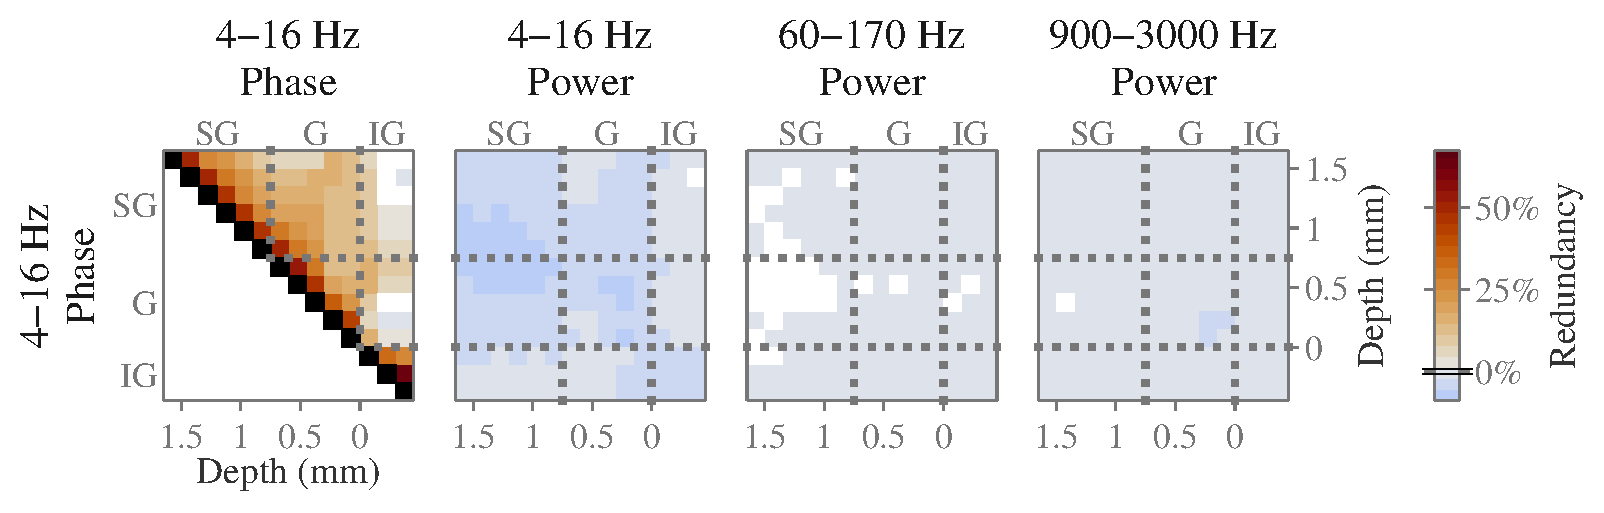
\includegraphics[scale=.5]{redundancy-cxschn/bndflt4-1-pcred-none-avg-lag=0s_paper.eps}
}
\\
\subfloat[Signal correlation\label{fig:lam_signal_corr_depth}]{
    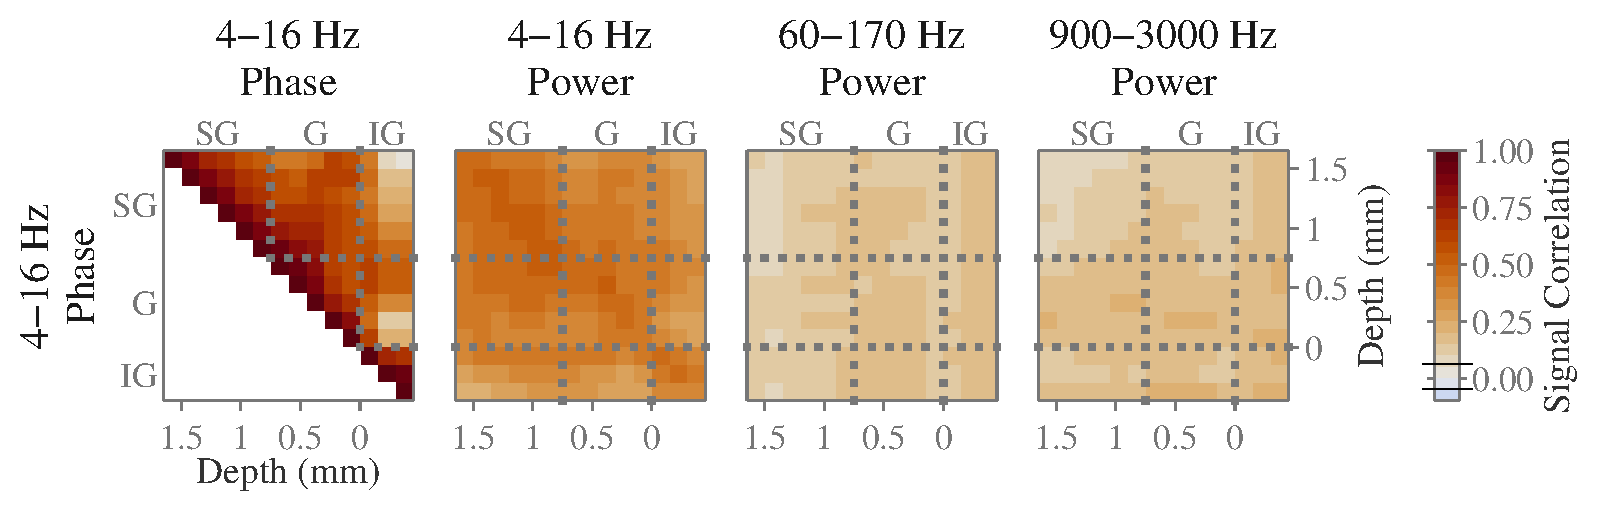
\includegraphics[scale=.5]{noisesigcorr/bndflt4-1-signal-avg_paper.eps}
}
\\
\subfloat[Noise correlation\label{fig:lam_noise_corr_depth}]{
    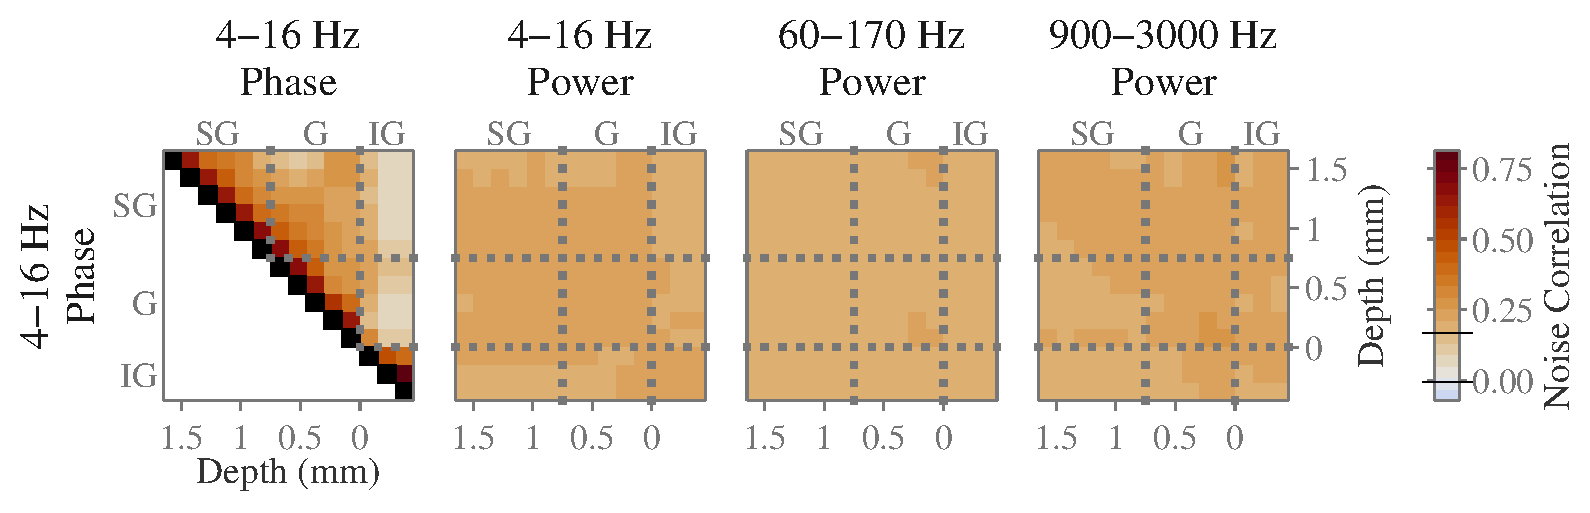
\includegraphics[scale=.5]{noisesigcorr/bndflt4-1-noise-avg_paper.eps}
}
\caption{
\textit{Redundancy of \SI{4}{16}{Hz} \ac{CSD} phase with \SI{4}{16}{Hz} power, \SI{60}{170}{Hz} power and \ac{MUA}.}
\protect\subref{fig:lam_signal_red_depth}:~Redundancy.
\protect\subref{fig:lam_signal_corr_depth}:~Signal correlation.
\protect\subref{fig:lam_noise_corr_depth}:~Noise correlation.
}
\label{fig:lam_noisesignal_corr_depth}
\end{figure}


%-------------------------------------------------------------------------------
\subsection{Information about scene cuts}
%-------------------------------------------------------------------------------

Method similar to \autoref{sec:lam_scnchg_method}.

\begin{figure}[htbp]
\centering
% \hspace*{\fill}
% \subfloat[][As a function the duration after the scene cut horizon threshold.\label{fig:lam_phs_scnchg_dur}]{%
%     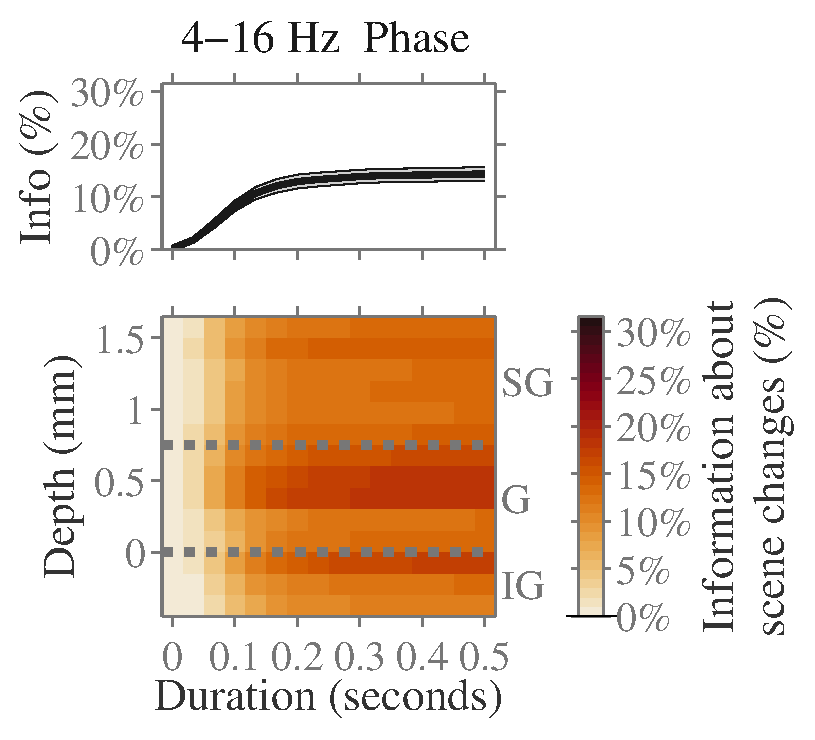
\includegraphics[scale=.5]{%
% scnchg/depth_v_scenecut-info_scnchg-dist_duration_avg_4-16Hz_phase.eps}}
% \hspace*{\fill}\hspace{.2cm}\hspace*{\fill}
% \subfloat[][Across a range of cortical frequencies.\label{fig:lam_phs_scnchg_frq}]{%
    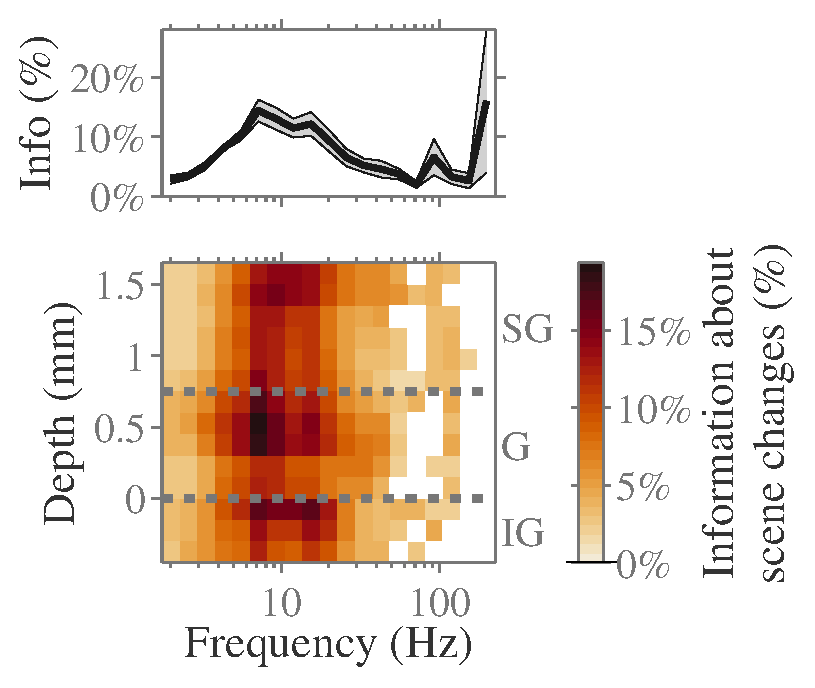
\includegraphics[scale=.5]{%
scnchg/frq-phase_v_depth_scenecut-info_scnchg-dist_0.200s_avg.eps}
% }
% \hspace*{\fill}
%
\caption{%
\textit{Information about the presence of scene cuts.}
We computed the information about scene cuts as described in \autoref{sec:lam_scnchg_method}, and for each session expressed this as a proportion of the total information present before averaging across recording sessions.
% \protect\subref{fig:lam_phs_scnchg_dur}: Information across the cortical depth for \SIrange{4}{16}{Hz} phase, averaged over \num{6} sessions.
Information values which were not significantly different from the bootstrap distribution are shown in white, with the median threshold for significance indicated by a black line across the colour bar.
Above, the average percentage of information explained by scene cuts over all cortical recording sites is shown, with the standard error across sessions indicated by the shaded region.

Information about scene cuts contained in a range of \ac{CSD} frequencies, in which we only considered the time since the last scene cut for the \SI{0.2}{\second} immediately following each.
}%
\label{fig:lam_phs_scnchg}
%
\end{figure}

The fraction of information contained in the \ac{CSD} which is explained by scene transitions in the movie is smaller for the phase (\autoref{fig:lam_phs_scnchg}) than the power (\autoref{fig:lam_scnchg}).
However, this is because the phase encodes more information about the stimulus than the power does.
Observing the phase of the oscillation provides us with more information about the timing of scene cuts than observing the power of the oscillation.


%-------------------------------------------------------------------------------
\subsection{Information about scene cuts}
%-------------------------------------------------------------------------------

Similar to \autoref{sec:lam_spatmf}, with method given in \autoref{sec:lam_tmf_method}.

\begin{figure}[htbp]
\centering
    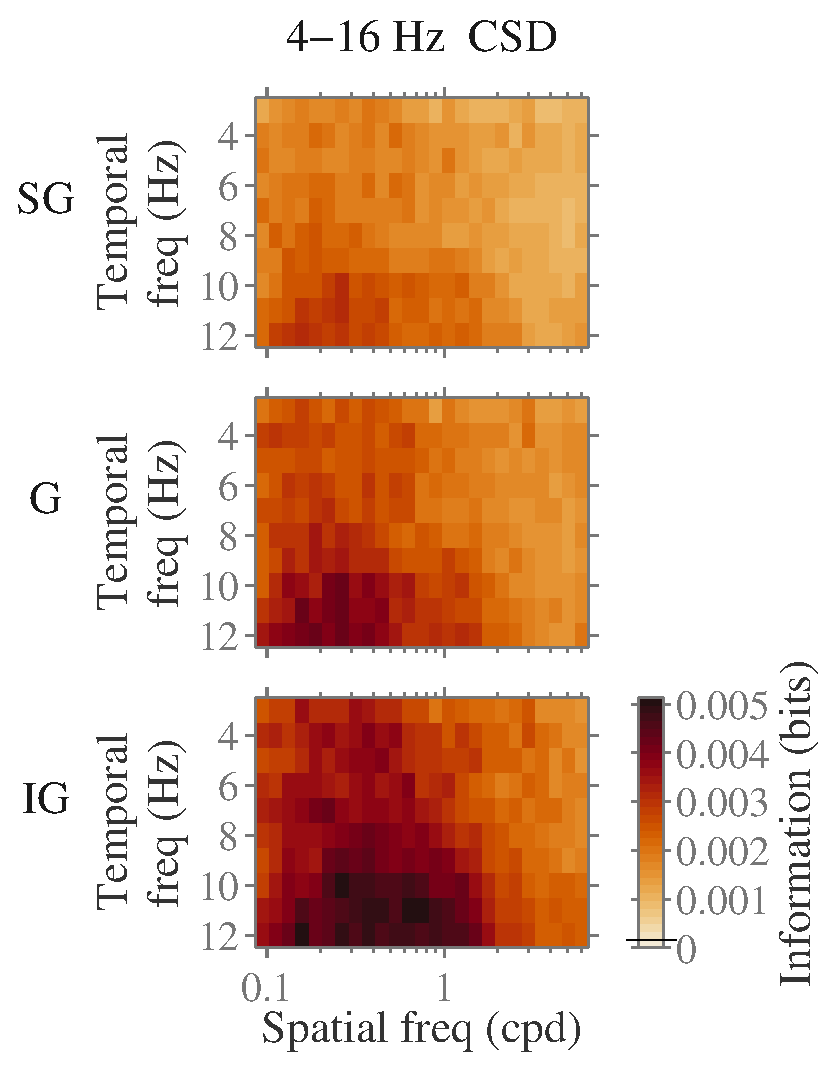
\includegraphics[scale=.5]{%
spatmf/tmf-v-spares-sggig-avg-spatmf2_4-16Hz_phase.eps}
\caption{%
Text
}%
\label{fig:lam_phs_spatmf}
%
\end{figure}


%-------------------------------------------------------------------------------


% %-------------------------------------------------------------------------------
% \subsubsection{Cross frequency phase vs power}
%
% \begin{figure}[htbp]
%     \centering
%     \subfloat[\label{fig:lam_cxfrq_powerphase_info_red_hm}]{
%         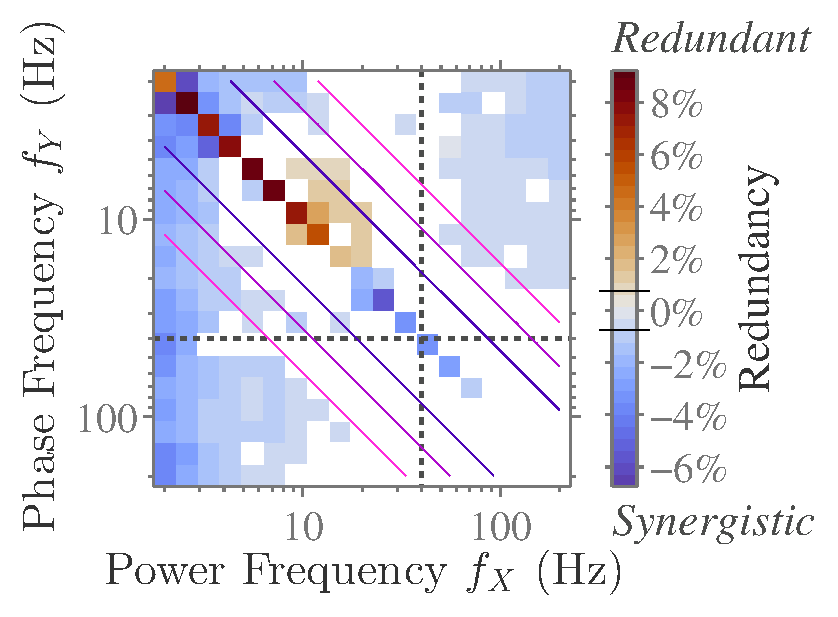
\includegraphics[scale=.5]{redundancy-cxsfrq/cxsfrq-pcred_phase-power_avg-log.eps}
% }
%     \\
%     \subfloat[\label{fig:lam_cxfrq_powerphase_info_red_bar}]{
%         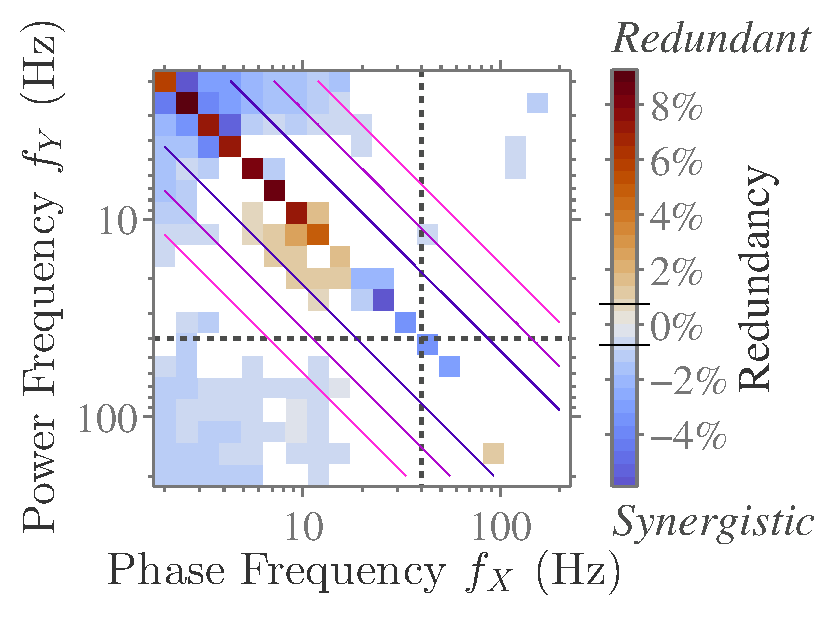
\includegraphics[scale=.5]{redundancy-cxsfrq/cxsfrq-pcred_power-phase_avg-log.eps}
% }
%     \caption{
% Redundancy between frequencies.
% }
% \label{fig:lam_cxfrq_powerphase_info_red}
% \end{figure}
%
%
%
% \begin{figure}[htbp]
%     \centering
%     \subfloat[\label{fig:lam_cxfrq_powerphase_info_gain_hm}]{
%         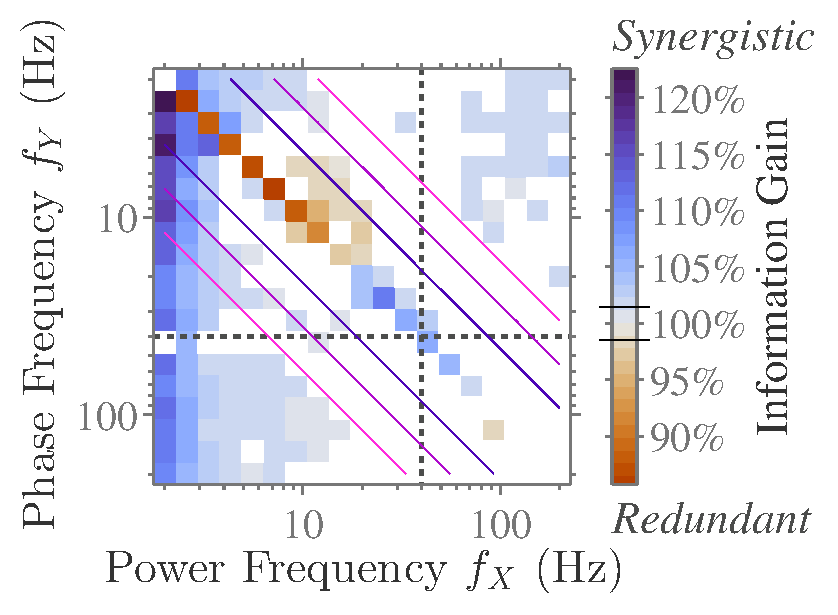
\includegraphics[scale=.5]{redundancy-cxsfrq/cxsfrq-pcgain-i2d2_phase-power_avg-log.eps}
% }
%     \\
%     \subfloat[\label{fig:lam_cxfrq_powerphase_info_gain_bar}]{
%         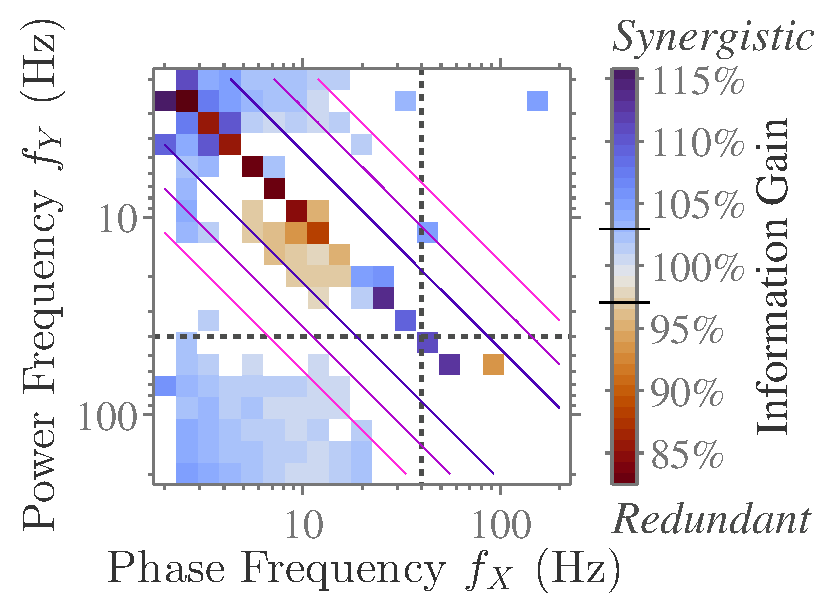
\includegraphics[scale=.5]{redundancy-cxsfrq/cxsfrq-pcgain-i2d2_power-phase_avg-log.eps}
% }
%     \caption{
% Information gain between frequencies.
% }
% \label{fig:lam_cxfrq_powerphase_info_gain}
% \end{figure}
%
% \begin{figure}[htbp]
%     \centering
%     \hspace*{\fill}
%     \subfloat[Signal correlation\label{fig:lam_signal_corr_phase_power}]{
%         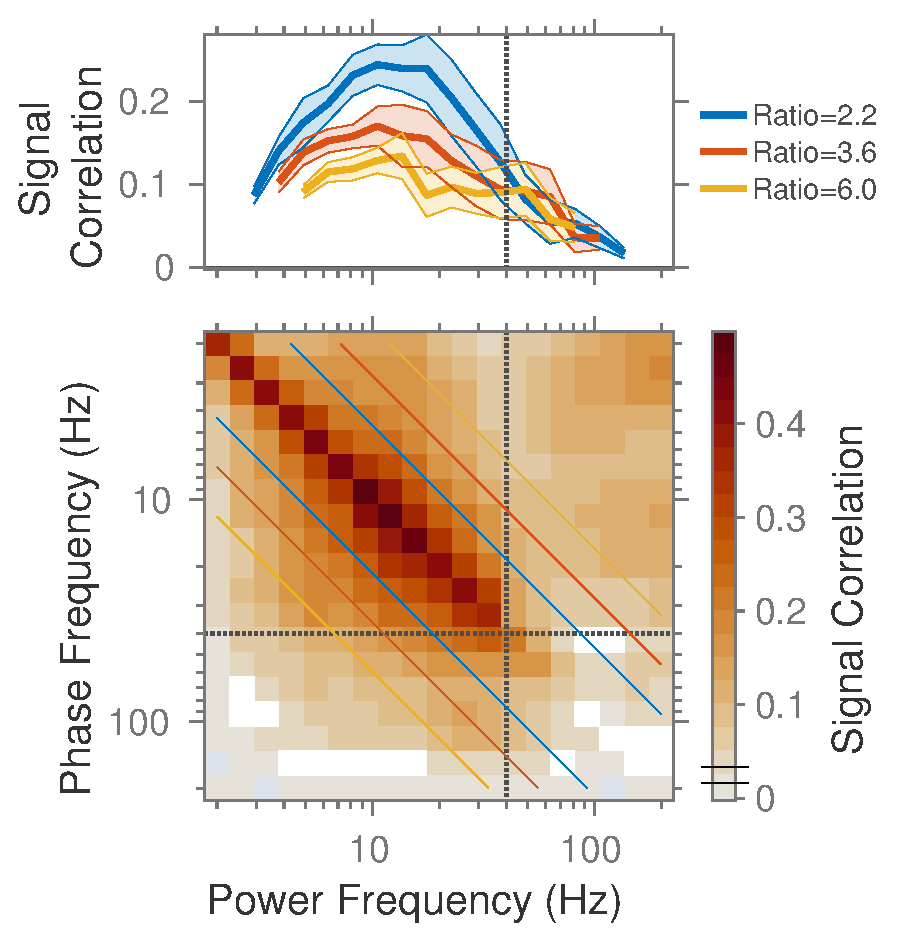
\includegraphics[scale=.45]{noisesigcorr/cxsfrq-signal-phase-power-avg-log.eps}
% }
%     \hspace*{\fill}\hspace{.2cm}\hspace*{\fill}
%     \subfloat[Noise correlation\label{fig:lam_noise_corr_phase_power}]{
%         %\includegraphics[scale=.45]{noisesigcorr/cxsfrq-noise-phase-power-avg-log.eps}
%         <code running>
% }
%     \hspace*{\fill}
%     \caption{Phase correlation with power
% \protect\subref{fig:lam_signal_corr_phase_power}:~Signal correlation.
% \protect\subref{fig:lam_noise_corr_phase_power}:~Noise correlation.
% }
% \label{fig:lam_noisesignal_corr_phase_power}
% \end{figure}


%-------------------------------------------------------------------------------
\FloatBarrier
\subsection{Phase synchrony, \SIrange{4}{16}{Hz}}
%-------------------------------------------------------------------------------

% \begin{figure}[htbp]
%     \centering
%     \hspace*{\fill}
%     \subfloat[Movie driven\label{fig:lam_phasestats_alpha_line_csd_movie}]{
%         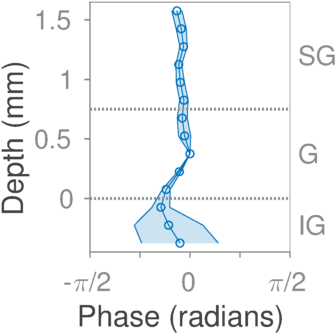
\includegraphics[scale=.45]{phasestats/movie1_Csd_phs4-16_dPhsTracebnd_5mean.png}
% }
%     \hspace*{\fill}\hspace{.2cm}\hspace*{\fill}
%     \subfloat[Spontaneous\label{fig:lam_phasestats_alpha_line_csd_spont}]{
%         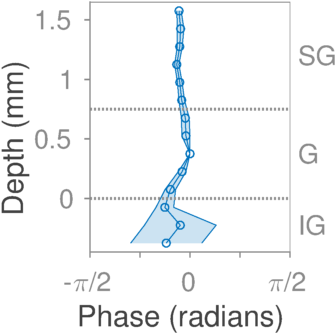
\includegraphics[scale=.45]{phasestats/spont_Csd_phs4-16_dPhsTracebnd_5mean.png}
% }
%     \hspace*{\fill}
%     \caption{Phase correlation, \SIrange{4}{16}{Hz}.
% \protect\subref{fig:lam_phasestats_alpha_line_csd_movie}:~Movie driven.
% \protect\subref{fig:lam_phasestats_alpha_line_csd_spont}:~Spontaneous.
% }
% \label{fig:lam_phasestats_alpha_line_csd}
% \end{figure}

% \begin{figure}[htbp]
%     \centering
%     \hspace*{\fill}
%     \subfloat[Movie driven\label{fig:lam_phasestats_alpha_hist_csd_movie}]{
%         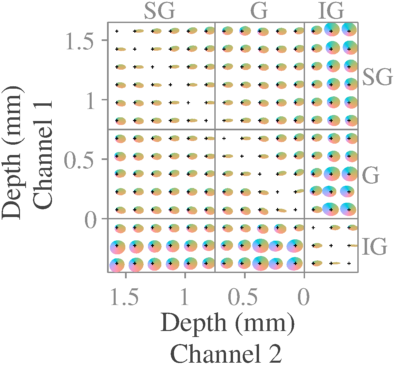
\includegraphics[scale=.45]{phasestats/movie1_Csd_phs4-16_dPhs_hist_5mean.png}
% }
%     \hspace*{\fill}\hspace{.2cm}\hspace*{\fill}
%     \subfloat[Spontaneous\label{fig:lam_phasestats_alpha_hist_csd_spont}]{
%         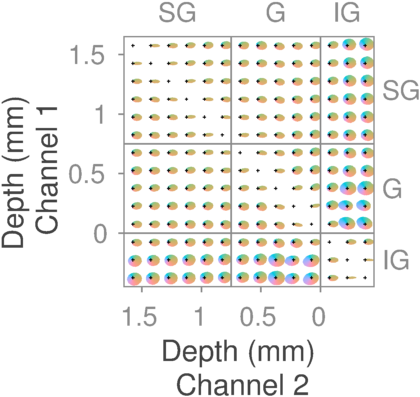
\includegraphics[scale=.45]{phasestats/spont_Csd_phs4-16_dPhs_hist_5mean.png}
% }
%     \hspace*{\fill}
%     \caption{Phase correlation, \SIrange{4}{16}{Hz}.
% \protect\subref{fig:lam_phasestats_alpha_hist_csd_movie}:~Movie driven.
% \protect\subref{fig:lam_phasestats_alpha_hist_csd_spont}:~Spontaneous.
% }
% \label{fig:lam_phasestats_alpha_hist_csd}
% \end{figure}


\begin{figure}[htbp]
    \centering
    \hspace*{\fill}
    \subfloat[Movie driven\label{fig:lam_phasestats_alpha_combo_csd_movie}]{
        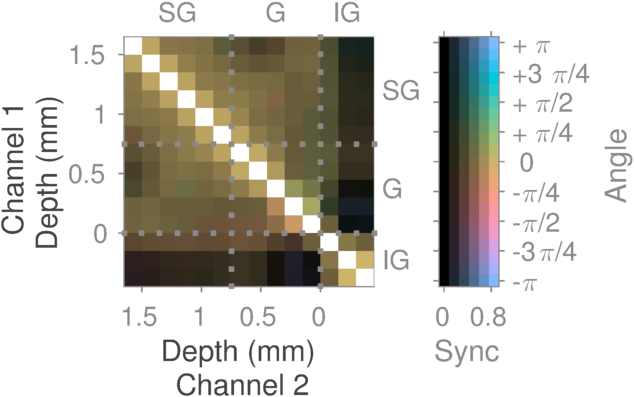
\includegraphics[scale=.45]{phasestats/movie1_Csd_phs4-16_dPhs_combo_5mean.png}
}
    \hspace*{\fill}\hspace{.2cm}\hspace*{\fill}
    \subfloat[Spontaneous\label{fig:lam_phasestats_alpha_combo_csd_spont}]{
        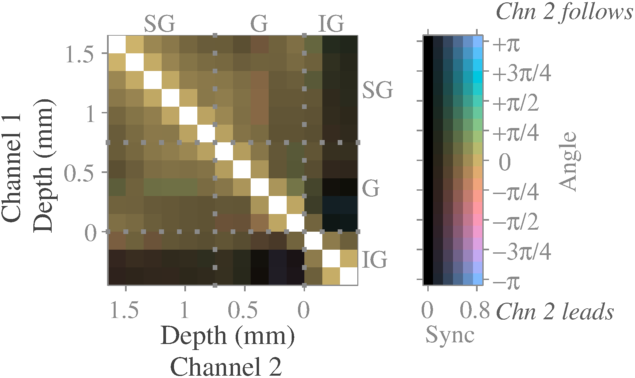
\includegraphics[scale=.45]{phasestats/spont_Csd_phs4-16_dPhs_combo_5mean.png}
}
    \hspace*{\fill}
    \caption{Phase correlation, showing phase offset and synchronicity \SIrange{4}{16}{Hz}.
\protect\subref{fig:lam_phasestats_alpha_combo_csd_movie}:~Movie driven.
\protect\subref{fig:lam_phasestats_alpha_combo_csd_spont}:~Spontaneous.
}
\label{fig:lam_phasestats_alpha_combo_csd}
\end{figure}


\begin{figure}[htbp]
    \centering
    \hspace*{\fill}
    \subfloat[Movie driven\label{fig:lam_phasestats_alpha_summary_csd_movie}]{
        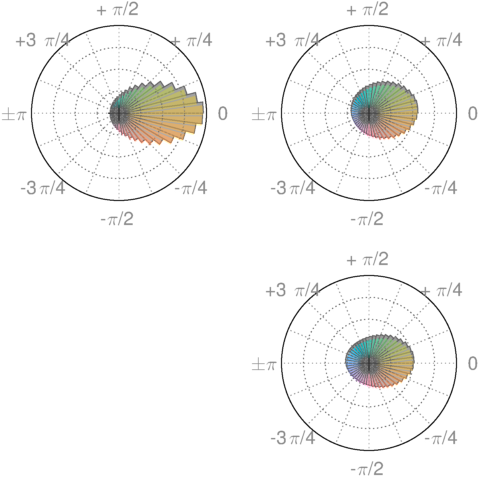
\includegraphics[scale=.45]{phasestats/movie1_Csd_simplephs4-16_dPhs_hist.png}
}
    \hspace*{\fill}\hspace{.2cm}\hspace*{\fill}
    \subfloat[Spontaneous\label{fig:lam_phasestats_alpha_summary_csd_spont}]{
        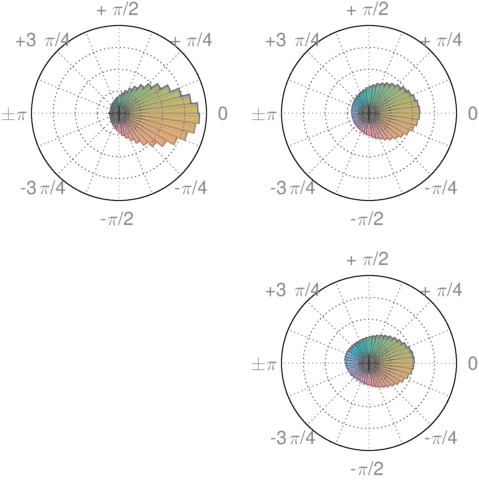
\includegraphics[scale=.45]{phasestats/spont_Csd_simplephs4-16_dPhs_hist.png}
}
    \hspace*{\fill}
    \caption{Phase correlation, summary by region, \SIrange{4}{16}{Hz}.
\protect\subref{fig:lam_phasestats_alpha_summary_csd_movie}:~Movie driven.
\protect\subref{fig:lam_phasestats_alpha_summary_csd_spont}:~Spontaneous.
}
\label{fig:lam_phasestats_alpha_summary_csd}
\end{figure}


%-------------------------------------------------------------------------------
\FloatBarrier
\subsection{Phase synchrony, \SIrange{60}{170}{Hz}}
%-------------------------------------------------------------------------------

% \begin{figure}[htbp]
%     \centering
%     \hspace*{\fill}
%     \subfloat[Movie driven\label{fig:lam_phasestats_gamma_line_csd_movie}]{
%         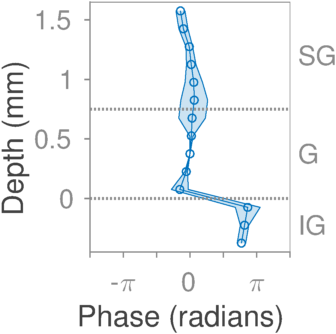
\includegraphics[scale=.45]{phasestats/movie1_Csd_phs60-170_dPhsTracebnd_5mean.png}
% }
%     \hspace*{\fill}\hspace{.2cm}\hspace*{\fill}
%     \subfloat[Spontaneous\label{fig:lam_phasestats_gamma_line_csd_spont}]{
%         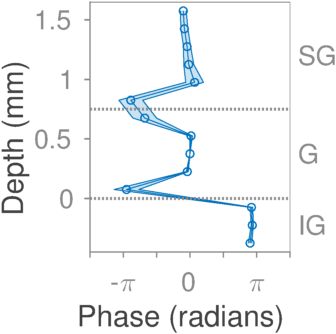
\includegraphics[scale=.45]{phasestats/spont_Csd_phs60-170_dPhsTracebnd_5mean.png}
% }
%     \hspace*{\fill}
%     \caption{Phase correlation, \SIrange{60}{170}{Hz}.
% \protect\subref{fig:lam_phasestats_gamma_line_csd_movie}:~Movie driven.
% \protect\subref{fig:lam_phasestats_gamma_line_csd_spont}:~Spontaneous.
% }
% \label{fig:lam_phasestats_gamma_line_csd}
% \end{figure}

% \begin{figure}[htbp]
%     \centering
%     \hspace*{\fill}
%     \subfloat[Movie driven\label{fig:lam_phasestats_gamma_hist_csd_movie}]{
%         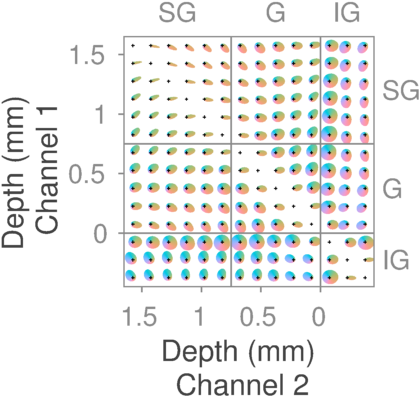
\includegraphics[scale=.45]{phasestats/movie1_Csd_phs60-170_dPhs_hist_5mean.png}
% }
%     \hspace*{\fill}\hspace{.2cm}\hspace*{\fill}
%     \subfloat[Spontaneous\label{fig:lam_phasestats_gamma_hist_csd_spont}]{
%         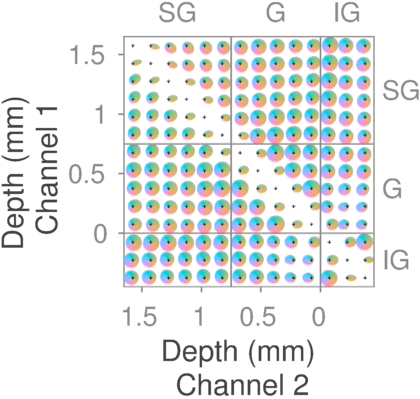
\includegraphics[scale=.45]{phasestats/spont_Csd_phs60-170_dPhs_hist_5mean.png}
% }
%     \hspace*{\fill}
%     \caption{Phase correlation, \SIrange{60}{170}{Hz}.
% \protect\subref{fig:lam_phasestats_gamma_hist_csd_movie}:~Movie driven.
% \protect\subref{fig:lam_phasestats_gamma_hist_csd_spont}:~Spontaneous.
% }
% \label{fig:lam_phasestats_gamma_hist_csd}
% \end{figure}


\begin{figure}[htbp]
    \centering
    \hspace*{\fill}
    \subfloat[Movie driven\label{fig:lam_phasestats_gamma_combo_csd_movie}]{
        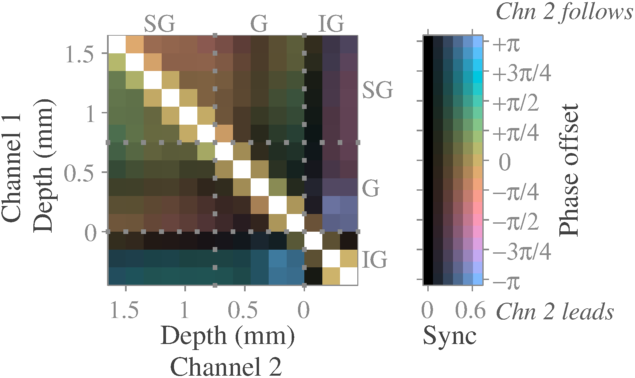
\includegraphics[scale=.45]{phasestats/movie1_Csd_phs60-170_dPhs_combo_5mean.png}
}
    \hspace*{\fill}\hspace{.2cm}\hspace*{\fill}
    \subfloat[Spontaneous\label{fig:lam_phasestats_gamma_combo_csd_spont}]{
        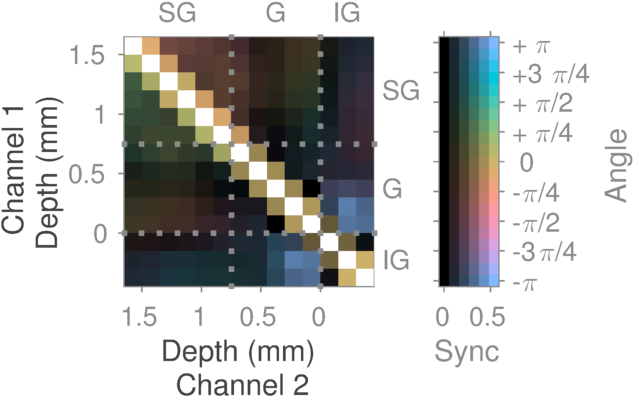
\includegraphics[scale=.45]{phasestats/spont_Csd_phs60-170_dPhs_combo_5mean.png}
}
    \hspace*{\fill}
    \caption{Phase correlation, showing phase offset and synchronicity \SIrange{60}{170}{Hz}.
\protect\subref{fig:lam_phasestats_gamma_combo_csd_movie}:~Movie driven.
\protect\subref{fig:lam_phasestats_gamma_combo_csd_spont}:~Spontaneous.
}
\label{fig:lam_phasestats_gamma_combo_csd}
\end{figure}


\begin{figure}[htbp]
    \centering
    \hspace*{\fill}
    \subfloat[Movie driven\label{fig:lam_phasestats_gamma_summary_csd_movie}]{
        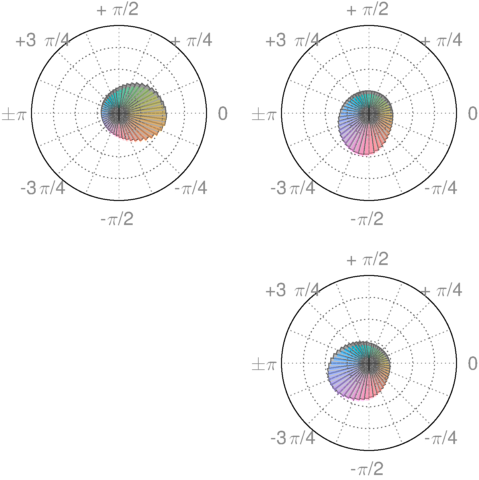
\includegraphics[scale=.45]{phasestats/movie1_Csd_simplephs60-170_dPhs_hist.png}
}
    \hspace*{\fill}\hspace{.2cm}\hspace*{\fill}
    \subfloat[Spontaneous\label{fig:lam_phasestats_gamma_summary_csd_spont}]{
        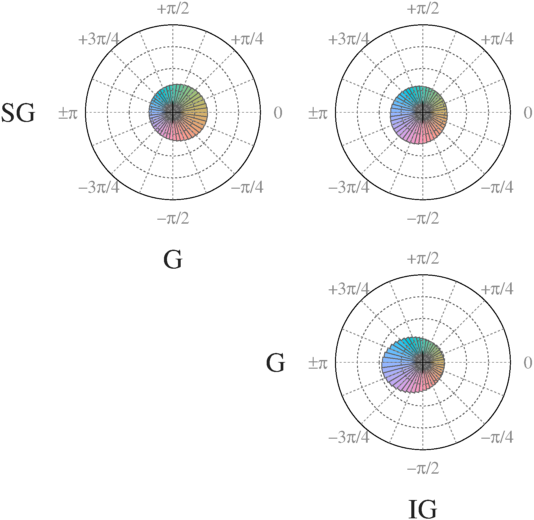
\includegraphics[scale=.45]{phasestats/spont_Csd_simplephs60-170_dPhs_hist.png}
}
    \hspace*{\fill}
    \caption{Phase correlation, summary by region, \SIrange{60}{170}{Hz}.
\protect\subref{fig:lam_phasestats_gamma_summary_csd_movie}:~Movie driven.
\protect\subref{fig:lam_phasestats_gamma_summary_csd_spont}:~Spontaneous.
}
\label{fig:lam_phasestats_gamma_summary_csd}
\end{figure}


%-------------------------------------------------------------------------------
\FloatBarrier
\subsection{Layer 1 \SIrange{60}{170}{Hz} amplitude is coupled to L5 \SIrange{4}{16}{Hz} phase}
%-------------------------------------------------------------------------------

Above, in section ``Information redundancy across depth'', we showed that high and low \ac{CSD} frequencies contain independent information to each other (\autoref{fig:lam_cxfrq_info}).
We found the power in the two bands to be independent, but it remains possible that there is a relationship between the phase of the low-frequency band and the power of the high-frequency band.
To investigate this possibility, we examined the cross-frequency coupling between the low-frequency phase and high-frequency oscillation amplitude.

Our observations showed that there is a spatially localised coupling between the \SIrange{4}{16}{Hz} phase of both lower-\ac{G} and mid-\ac{IG} with the amplitude of \SIrange{60}{170}{Hz} oscillations in upper-\ac{SG} (\autoref{fig:lam_8}).
Additionally, in both \ac{G} and \ac{IG} there is a coupling between the local \SIrange{4}{16}{Hz} phase and the local \SIrange{60}{170}{Hz} amplitude.

The same relationship was discovered to hold both for spontaneous activity and stimulus-driven recordings, and our findings are in agreement with previous work \citep{Spaak2012}.

\begin{figure}[htbp]
\centering 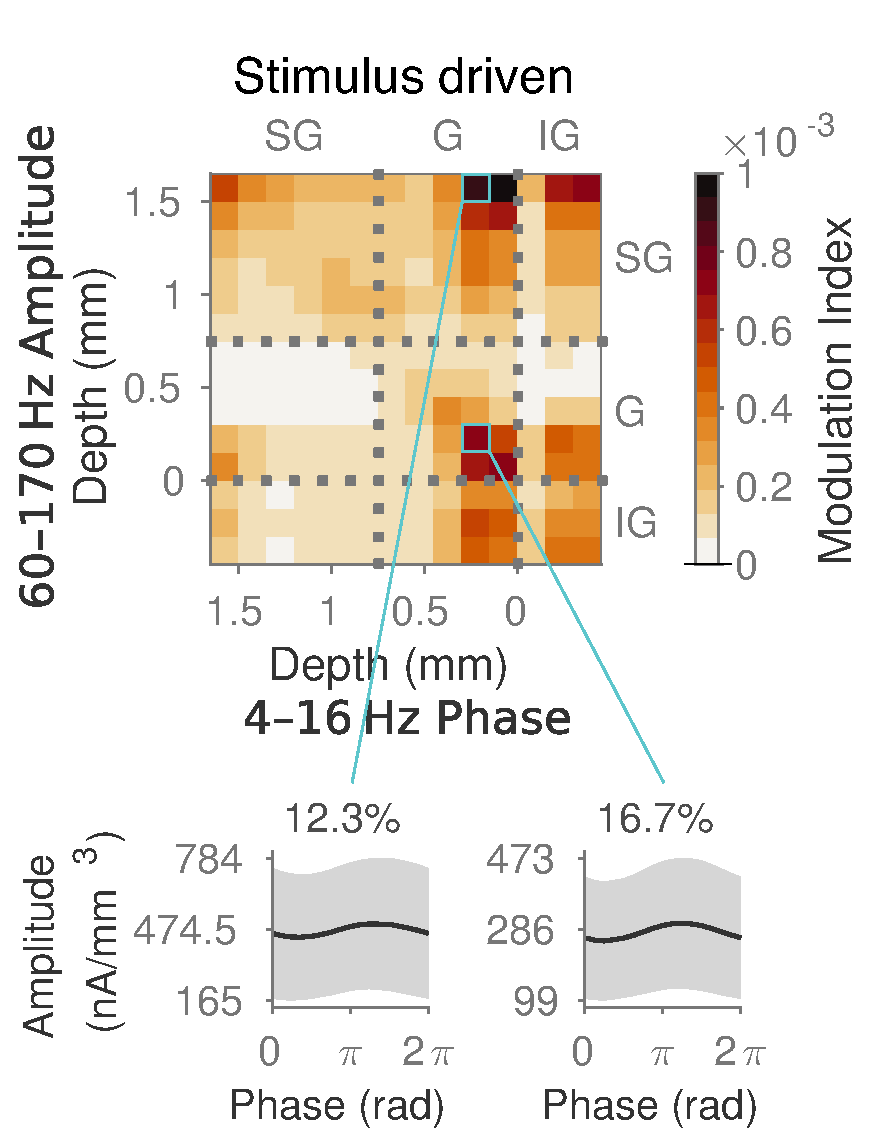
\includegraphics[width=\columnwidth]{cfc/fig8A.eps}
%
\caption{%
\textit{Cross-frequency phase-amplitude coupling}
Phase-amplitude modulation index between low frequency (\SIrange{4}{16}{Hz}) phase and high frequency (\SIrange{60}{170}{Hz}) amplitude (A: movie driven activity; B: spontaneous activity).
Mean of \num{5} sessions.
C and D: Amplitude as a function of binned phase for an example session (\sesname{H05391}), for \ac{IG}$\rightarrow$\ac{IG} coupling (left) and \ac{IG}$\rightarrow$\ac{SG} coupling (right).}%
\label{fig:lam_8}
%
\end{figure}


%-------------------------------------------------------------------------------
\section{Discussion}
%-------------------------------------------------------------------------------
